\documentclass{beamer}
\usepackage{graphicx}
\usetheme{Singapore}

\def\UrlBreaks{\do\/\do-} % URL breaks
\setbeamertemplate{caption}[numbered] % number figures
\setbeamertemplate{bibliography item}{\insertbiblabel} % bibliography numbers
\makeatletter
\newcommand*{\rom}[1]{\expandafter\@slowromancap\romannumeral #1@}
\makeatother

\title{Research Project Last-Layer Variational Inference}
\author{Philipp von Bachmann}
\institute{University of Tübingen}
\date{\today}



\begin{document}
        \begin{frame}
            \titlepage
        \end{frame}
        
        \section{Recap}
        \begin{frame}
            \frametitle{Where we left of}
            \begin{columns}
                \begin{column}{0.5\textwidth}
                    \begin{itemize}
                        \item Setup: Deep Learning, learn weight distribution with Variational Inference
                        \item Use Gaussian distributions for prior and variational
                        \item Initally good results for Regression and mixed results for Classification
                    \end{itemize}
                \end{column}
                \begin{column}{0.5\textwidth}
                    \begin{figure}
                        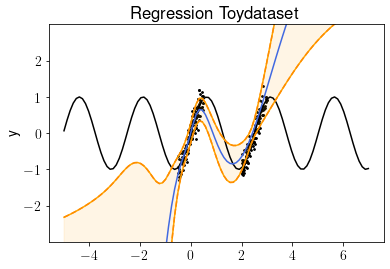
\includegraphics[width=\textwidth]{images/Regression/Toydataset.png}
                    \end{figure}
                \end{column}
            \end{columns}
        \end{frame}
        
        \section{Closed-form Solutions}
        \begin{frame}
            \frametitle{Regression}
            \begin{itemize}
                \item The expected log-likelihood $\mathbb{E}_{q_{\phi}(\theta)}[\log{p(y \vert f_{\theta}(x))}]$ has a closed form solution in the Regression case.
                \item The solution gives a lower bound for approximation (like MC) on ELBO in practice.
                \item This leads to faster convergence.
            \end{itemize}
            \begin{figure}
                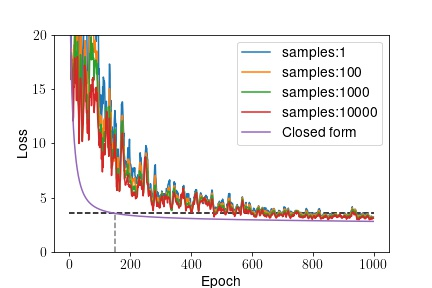
\includegraphics[width=0.7\textwidth]{images/Regression/CFvsMC.jpg}
            \end{figure}
        \end{frame}

        \begin{frame}
            \frametitle{Classification}
            \begin{itemize}
                \item No closed-form solution
                \item However multiple approximations like Jennsen, Bohning
                \item Perform worse than Monte-Carlo
            \end{itemize}
        \end{frame}
        
        \section{Last-Layer vs FUll}
        \begin{frame}
            \frametitle{Regression}
            \begin{itemize}
                \item Full layer has better solution, especially higher in-between uncertainty
                \item Last-Layer converges way faster 
            \end{itemize}
            \begin{columns}
                \begin{column}{0.5\textwidth}
                    \begin{figure}
                        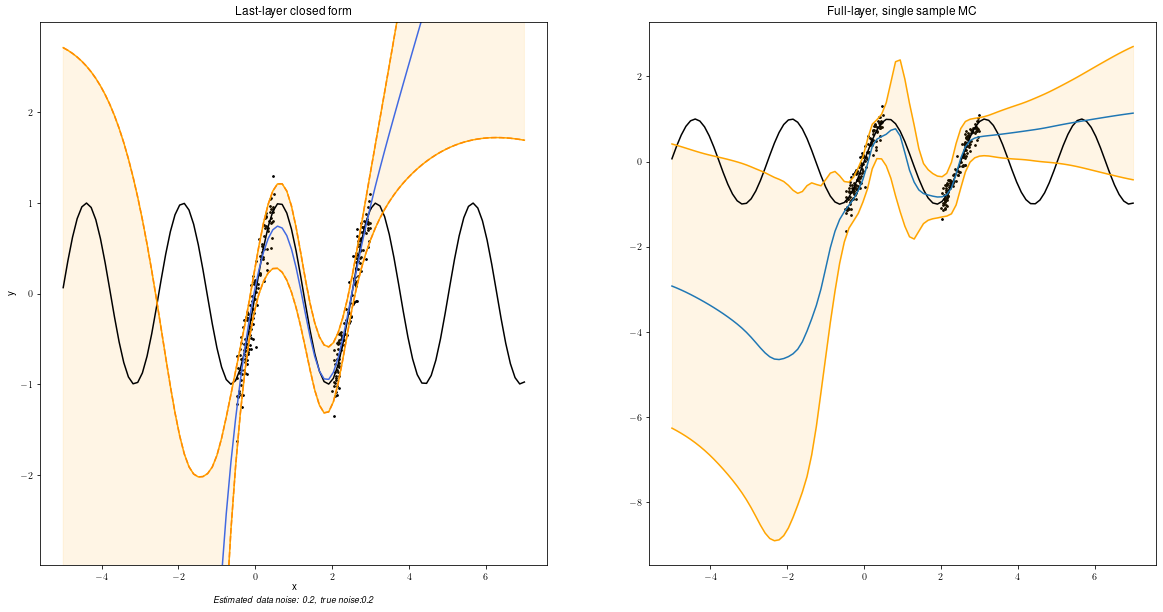
\includegraphics[width=\textwidth]{images/RegressionLLvsFULL.png}
                    \end{figure}
                \end{column}
                \begin{column}{0.5\textwidth}
                    \begin{figure}
                        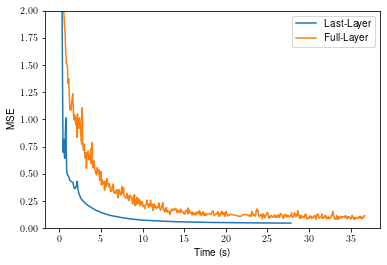
\includegraphics[width=\textwidth]{images/RegressionLLvsFullEpoch.png}
                    \end{figure}
                \end{column}
            \end{columns}
        \end{frame}

        \begin{frame}
            \frametitle{Classification: MNIST}
            \begin{figure}
                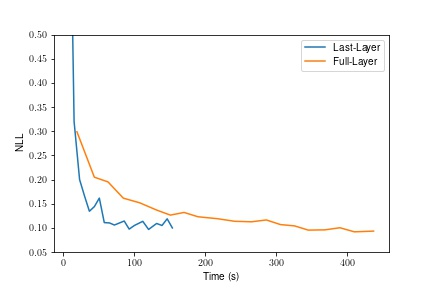
\includegraphics[width=\textwidth]{images/Classification/LLvsFull.jpg}
            \end{figure}
        \end{frame}


        \section{VI vs Laplace}

        \begin{frame}
            \frametitle{Equivalence of VI and Laplace}
            \begin{itemize}
                \item Claim: Laplace approximation is equivalent to Natural Gradient Descent for VI
                \item Bayesian Learning Rule which can be derived from VI:     
                    \begin{equation}
                        \lambda_{t+1} \leftarrow \lambda_{t} - \rho \tilde{\nabla}_\lambda E_{q_t}[l(\theta) - H(q_t)]
                    \end{equation}
                    where $\lambda$ natural parameters, $\tilde{\nabla}$ natural gradient
                \item If $q = \mathcal{N}(m, S^{-1})$, the update for precision $S$ becomes:
                    \begin{equation}
                        S_{t+1} = (1 - \rho_t) S_t + \rho_t E_{q_t}[\nabla^2_\theta l(\theta)]
                    \end{equation}
                \item Equivalent to online-computation of the Hessian
            \end{itemize}
        \end{frame}

        \begin{frame}
            Laplace initializations
        \end{frame}
        
        


        % \begin{frame}
        %     \frametitle{Regression}
        %     add regression comparison of kernels here
        %     \begin{figure}
        %         \includegraphics[width=0.8\textwidth]{images/Regression/FullCov.jpg}
        %     \end{figure}
        % \end{frame}

        % \begin{frame}
        %     \frametitle{Classification: Two Moons}
        %     add non-bayesian vs best kernel comparison here, maybe vs laplace?
        %     \begin{columns}
        %         \column{0.5\textwidth}
        %         \begin{figure}
        %             \includegraphics[width=\textwidth]{images/TowMoons/Baseline.jpg}
        %         \end{figure}
        %         \column{0.5\textwidth}
        %         \begin{figure}
        %             \includegraphics[width=\textwidth]{images/TowMoons/Diagonal.jpg}
        %         \end{figure}
        %     \end{columns}
        % \end{frame}








\end{document}
